%In the following, we 

%\color{blue}




%\revised{

This section describes the planning of our evaluation, having the {\em goal} of evaluating the performance of \CR. In Section~\ref{sec:Dataset}, we introduce the dataset exploited in our evaluation. The evaluation methodology and metrics are presented in Section~\ref{sec:methodology-metric}. Finally, Section~\ref{sec:ResearchQuestions} describes the research questions.


%ten equal parts, so-called folds
%We also exploited 
%was also exploited 

\begin{figure}[h!]
	\centering
	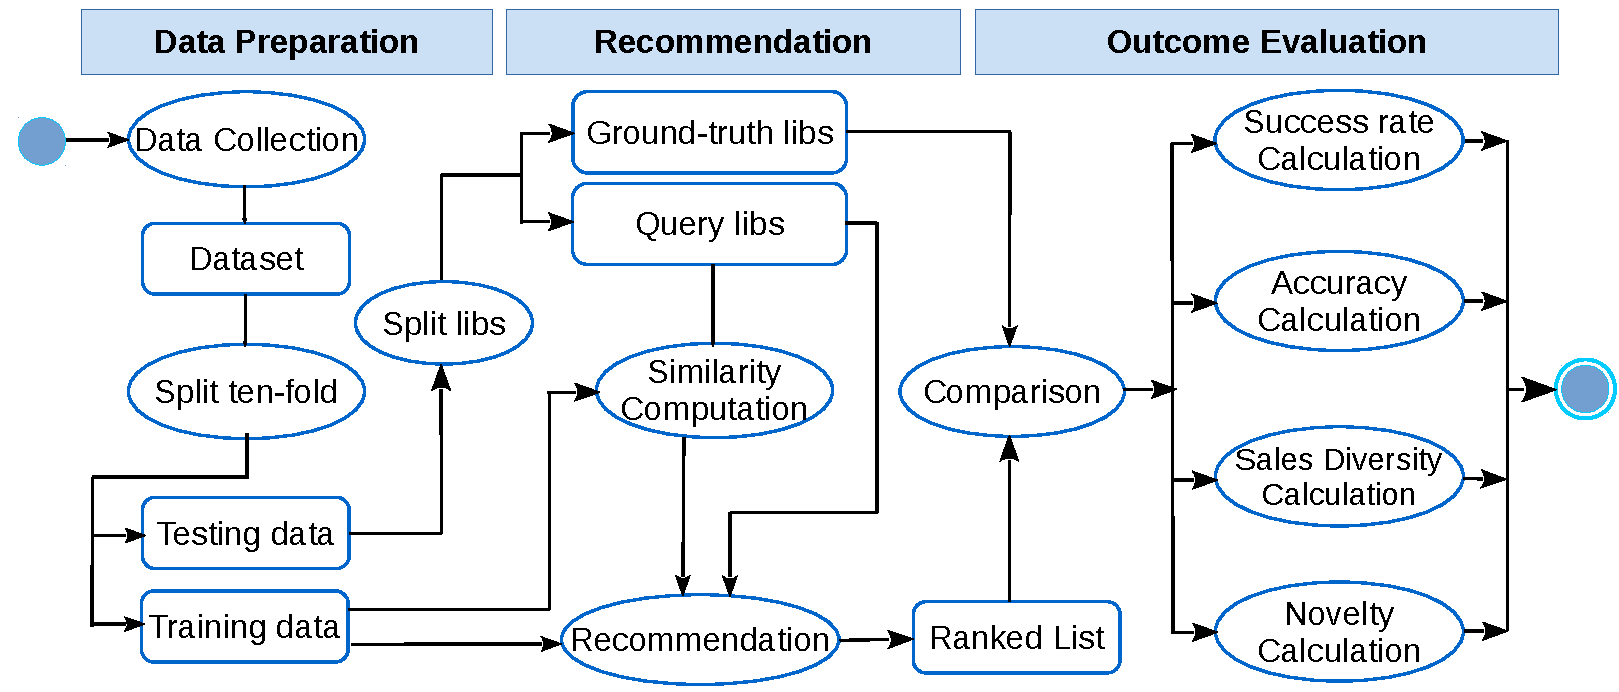
\includegraphics[width=\linewidth]{figs/EvaluationProcess.pdf}
	%\vspace{-.3cm}
	\caption{Evaluation Process.}
	\label{fig:EvaluationProcess}
	\vspace{-.3cm}
\end{figure}

The evaluation process is depicted in Fig.~\ref{fig:EvaluationProcess} and it consists of three consecutive phases,~\ie~\emph{Data Preparation},~\emph{Recommendation}, and~\emph{Outcome Evaluation}. We start with the \emph{Data Preparation} phase by creating a dataset from  GitHub projects. %Such datasets are used to assess the performances of \CR, but also to evaluate two of the baselines, \ie \LF and \LC. 
The dataset is then split into training and testing sets.  In the \emph{Recommendation} phase, given a project in the testing set, a portion of its topics is extracted as ground-truth data, and the remaining is used as query to compute similarity and recommendations. Finally, by the \emph{Outcome Evaluation} phase, we compare the recommendation results with those stored as ground-truth data to compute the quality metrics. All the aforementioned phases are  detailed in the rest of this section.


\subsection{Dataset Extraction} \label{sec:Dataset}


%\color{blue}

To evaluate the systems, we exploited a dataset with 6258 \GH repositories that use 15757 topics.

By means of the GitHub API \cite{githubAPI} we \emph{randomly} collected a dataset consisting of $6,258$ repositories. 
\CDS{Add how the dataset has been mined (\ie constraints in term of stars, forks, num of topic, etc)}
\JDR{Add Statistics}%Among these projects, only $7$ of them have been forked from other projects. Such original projects have been excluded from the dataset as their forked ones share highly similar libraries, and this may introduce bias in the recommendation outcomes. We represent the distribution of projects with respect to the number of forks, commits and pull requests in Fig.~\ref{fig:ForkCommitPull}. Most projects have a low number of pull requests, \ie lower than 100, however many of them have a large number of forks and commits. Forking is a means to contribute to the original repositories~\cite{Jiang:2017:WDF:3042021.3042043}. Furthermore, there is a strong correlation between forks and stars~\cite{7816479}, as it is further witnessed in Fig.~\ref{fig:ForkStarIssue}. A project with a high number of forks means that it gets attention from the OSS community. In this sense, having many forks can be considered as a sign of a well-maintained and well-received project. Meanwhile, as commits have an impact on the source code~\cite{8009930}, the number of commits is also a good indicator of how a project has been developed.
%}


%e mined dependency specification by means of \code{code.xml} or \code{.grad\-le} files.\footnote{The files \code{pom.xml} and with the extension \code{.gradle} are related to management of dependencies by means of Maven (\url{https://maven.apache.org/}) and Gradle (\url{https://gradle.org/}), respectively.} Fig.~\ref{fig:NumOfLibsD1} depicts the distribution of libraries across the projects. Most of the libraries in \code{D1} ($12,962$) are used by a small number of projects, and only $10$ libraries are extremely popular by being included in more than $200$ projects. By carefully investigating the dataset, we also see that most projects contain a small number of dependencies, \ie $48\%$ of the projects include less than $20$ libraries and just $15\%$ of them include more than $100$ libraries. \}


%\color{blue}
	\subsection{Evaluation Methodology and Metrics’ Definition}\label{sec:methodology-metric}
To assess the performance of \CR proposed approach, we applied ten-fold cross-validation, considering every time $9$ folds (each one contains $625$ projects) for training and the remaining one for testing. 
	For every testing project \emph{p}, a half of its topics are \emph{randomly} 
	taken out and saved as ground truth data, let us call them \emph{GT(p)}, which will be used to validate the recommendation outcomes. The other half are used 
	as testing topics or query, which are called \emph{\textbf{te}}, and serve 
	as input for \code{Similarity Computation} and \code{Recommendation}. %Though 	the ratio of query to ground-truth data can be arbitrarily set, we chose $50\%$ 	for two reasons: \emph{(i)} this value was used in the evaluation of the baselines in the original 	work~\cite{6671293},\cite{Ouni:2017:SSL:3032135.3032325},\cite{SAIED2018164}; 	and \emph{(ii)} no matter how big a query is, the most important thing is to 	use exactly the same amount of data when evaluating the systems. In a separate 	experiment discussed later in this paper, the ratio of query to ground-truth 	has been varied to investigate whether an increase in the amount of testing 	data helps improve CrossRec's overall performance.
%\color{black} 
The splitting mimics a real development process where a 
developer has already included some topics in the current project, \ie 
\emph{\textbf{te}} and waits for recommendations, that means additional topics to be incorporated. A recommender system is expected to provide her 
with the other half, \ie \emph{GT(p)}. %To ensure a reliable comparison between \LR and \CR, we performed cross-validation for both using exactly the same folds.


%====================================================================================================================================

%there are different ways to split the original data to produce training and testing sets, 
%training and test folds for each validation round.
%For each validation round, we use the same folds for testing and training by both systems.
%Also for a testing project, the same sets of testing libraries and ground-truth libraries are used for experiments on \LR and \CR. This is to make sure that exactly the same condition is applied in both systems, so as to precisely validate their performance. 
%The list of the projects together with the corresponding folds are publicly available in GitHub \cite{CROSSREC-DATA}.

%To aim for reproducibility, we published 
%\color{blue}\textbf{\emph{@Juri: Please help with this. Thanks!}} are freely available 
%\footnote{\CR implementation and dataset: \url{https://github.com/MSR18-CROSSREC/MSR18-CROSSREC}}
% the dataset as well as all the experimental results

%compared against the corresponding ground-truth data to compute the quality metrics. 
% (See Section \ref{sec:SimilarityComputation})
%, \ie \emph{recall rate}, \emph{accuracy}, \emph{sales diversity}, and \emph{novelty}. 
%This module performs the user-based collaborative-filtering technique on the set of \emph{k} similar projects and their corresponding sets of libraries to recommend libraries. The final outcome of this process is a ranked list of \emph{top-N} libraries which is then recommended to the input project.
%For \textbf{Validation} in Module $5$, the list of recommended libraries $REC(p)$ is compared against the set of ground-truth data \emph{GT(p)} extracted in Module $1$.
%then used to compute similarity between the testing project and all $1080$ projects using VsmSim. 
%To study the outcomes, first we consider \emph{recall rate@N} which was used as the only evaluation metric for \LR \cite{6671293}.
%Using these notations, 

%\color{black}


%====================================To justify the selection of the quality metrics in this paper====================================

% Among others, \emph{precision} and \emph{recall} are considered among the most suitable metrics for evaluating top-$N$ items of the recommendation outcomes \cite{Ostuni:2013:TRI:2507157.2507172}.

There are several metrics available to evaluate a ranked list of recommended items \cite{DBLP:conf/rweb/NoiaO15}. In the scope of this paper, \emph{success rate}, \emph{accuracy}, \emph{sales diversity}, and \emph{novelty} have been used to study the systems' performance as already proposed by Robillard \etal~\cite{Robillard:2014:RSS:2631387} and other studies~\cite{6671293},\cite{Nguyen:2015:ESP:2740908.2742141}. For a clear presentation of the metrics considered during the outcome evaluation, let us introduce the following notations:

\begin{itemize}[noitemsep,topsep=0pt]
	\item \emph{N} is the cut-off value for the ranked list;% of recommended libraries;
	\item \emph{k} is the number of neighbor projects exploited for the recommendation process;
	\item For a testing project \emph{p}, a half of its topics are extracted and used as the ground-truth data named as \emph{GT(p)};
	\item $REC(p)$ is the \emph{top-N} topics recommended to \emph{p}. It is a ranked list in descending order of real scores;%, with $REC_r(p)$ being the recommended library in the position $r$.		
	\item If a recommended tiopic $t \in REC(p)$ for a testing project $p$ is found in the ground truth of $p$ (\ie \emph{GT(p)}), hereafter we call this as a topic \textit{match} or \textit{hit}.	
\end{itemize}	


%================================================================================================================================================
%a comprehensive work on the application of recommender systems in Software Engineering. this work also 
%Di Noia \etal present a comprehensive description on how to evaluate a recommender system \cite{DBLP:conf/rweb/NoiaO15}. 
%With the aim of introducing recommendation techniques for the Semantic Web, Di Noia \etal address issues about the exploitation of Linked Data to build recommender systems .
%The metrics utilized to measure the recommendation outcomes are explained in the following. % is as follows
%================================================================================================================================================

%====================================To justify the selection of the quality metrics in this paper====================================

%There are several metrics available to evaluate a ranked list of recommendations \cite{DBLP:conf/rweb/NoiaO15}. Among others, \emph{precision} and \emph{recall} are considered among the most suitable metrics for evaluating a top-$N$ ranked list of items \cite{Ostuni:2013:TRI:2507157.2507172}. Together with a thoughtful discussion of various topics such as building recommender systems and presenting recommendations, Robillard \etal introduce various quality metrics for evaluating recommendation outcomes in Software Engineering, \eg \emph{precision} and \emph{recall}, \emph{confidence}, and \emph{serendipity}~\cite{robillard_recommendation_2014}. In the scope of this paper, to evaluate the recommendations by \LR and \CR, we opt for \emph{success rate}, \emph{accuracy}, \emph{sales diversity} and \emph{novelty} as already proposed in~\cite{robillard_recommendation_2014} and other studies~\cite{Nguyen:2015:ESP:2740908.2742141},\cite{6671293}.

If $REC_{N}(p)$ is the set of top-$N$ items and\\
 $match_{N}(p)=  GT(p) \bigcap REC_{N}(p) $ is the set of items in the \emph{top-N} list that match with those in the ground-truth data, then the metrics are defined as follows.

\paragraph{\textbf{Success rate@N}} Given a set of testing projects \emph{P}, this metric measures the rate at which a recommender system returns at least a topic match among \emph{top-N} items for every project $p \in P$ \cite{6671293}: %It is formally defined as given below:
\vspace{-.3cm}

\begin{equation} \label{eqn:RecallRate}
success\ rate@N=\frac{ count_{p \in P}( \left |  match_{N}(p) \right | > 0 ) }{\left | P \right |} %\times 100\%
%success\ rate@N=\frac{ count_{p \in P}( \left |  GT(p) \bigcap (\cup_{r=1}^{N} REC_{r}(p)) \right | > 0 ) }{\left | P \right |} 
\end{equation}

\noindent where the function \emph{count()} counts the number of times that the boolean expression specified in its parameter is \emph{true}.


\paragraph{\textbf{Accuracy}} Accuracy is considered as one of the most preferred \emph{quality indicators} for Information Retrieval applications \cite{Saracevic:1995:EEI:215206.215351}. However, \emph{success rate@N} does not reflect how accurate the outcome of a recommender system is. For instance, given only one testing project, there is no difference between a system that returns $1$ topic match out of $5$ and another system that returns all $5$ topic matches, since \emph{success rate@5} is $100\%$ for both cases (see Eq.~\eqref{eqn:RecallRate}). Thus, given a list of \emph{top-N} topics, \emph{precision@N} and \emph{recall@N} are utilized to measure the \emph{accuracy} of the recommendation results. \emph{precision@N} is the ratio of the \emph{top-N} recommended topics belonging to the ground-truth dataset, whereas \emph{recall@N} is the ratio of the ground-truth topics appearing in the \emph{N} recommended items \cite{Nguyen:2019:FRS:3339505.3339636},\cite{DiNoia:2012:LOD:2362499.2362501},\cite{Davis:2006:RPR:1143844.1143874}: %,Nguyen:2015:CRV:2942298.2942305 %}. A concrete definition for the metrics is given below \cite{

%\vspace{-.2cm}
% \cite{Saracevic:1995:EEI:215206.215351}

\begin{equation} \label{eqn:Precision}
precision@N = \frac{ \left |  match_{N}(p) \right | }{N}
%precision@N(p) = \frac{\sum_{r=1}^{N}\left |  GT(p) \bigcap REC_{r}(p) \right |}{N}
\end{equation}
%\vspace{-.1cm}
\begin{equation} \label{eqn:Recall}
recall@N = \frac{ \left |  match_{N}(p) \right | }{\left | GT(p) \right |}	
%recall@N(p) = \frac{\sum_{r=1}^{N}\left |  GT(p) \bigcap REC_{r}(p) \right |}{\left | GT(p) \right |}	
\end{equation}
%\vspace{-.1cm}

\paragraph{\textbf{Sales Diversity}} This term originates from the business domain where it is important to 
improve the coverage as also the distribution of products across customers, thereby increasing the 
chance that products will get sold by being introduced 
\cite{Vargas_sales_diversity_14}. Similarly, in the context 
of topic recommendation, \emph{sales diversity} indicates the ability of the system to suggest to 
projects as much topics as possible, as well as to disperse the concentration among all items, 
instead of focusing only on a specific set of topics \cite{Robillard:2014:RSS:2631387}. 
In the scope of this paper, \emph{catalog coverage} and \emph{entropy} are utilized to gauge 
\emph{sales diversity}. Let $T$ be the set of all 
topic available for recommendation, $\#rec(t)$ denote the number of projects getting topic 
$t$ as a recommendation, \ie $\#rec(t)=count_{p \in P}( \left |   REC_{N}(p)  \ni t  \right |  )$, $t \in T $, and $total$ denote the number of recommended items across all projects.
%Nguyen:2015:CRV:2942298.2942305,
%====================================================================================================================================
%.In the context of library recommendation, Sales diversity measures the ability of a recommender system to expose all libraries to projects so that can be recommended to a project
%, and \emph{Gini Index}. 
%. , \emph{entropy} is defined as follows
%To increase the possibility that all products can be sold by being recommended. 
%Sales diversity is defined as the statistical distribution of market shares of all products that are offered by an online vendor. The ability of a recommender system to provide its users with.
%\emph{Sales Diversity} means the ability of the system to. \emph{Sales Diversity} represents an important quality dimension for both business and user perspective, since improving the coverage of the items catalog and of the distributions of the items across the users may increase the sales and the user satisfaction \cite{}. %The term is borrowed from business where it is important to improve the range of products as well as the distribution of the products across the customers. Similarly in the context of library recommendation, 
%Sales diversity means that all or most products in the business catalog get purchased to some extent, rather than having sales concentrating around a few items. Sales diversity gets meaning in the context of recommendation in the sense that recommending a product exposes it to being sold. By link-ing recommendation to purchase in the analysis of diversity, “sales diversity” becomes a shorthand for “promoting sales diversity”.\cite{Vargas_sales_diversity_14}
%Catalog Coverage: and it is given below: %measures the ability of a recommender system to recommend as many items as possible. %Catalog coverage is the proportion of available items that the recommendation system recommends to users \cite{robillard_recommendation_2014}.
%====================================================================================================================================
%

\emph{Catalog coverage} measures the percentage of topic being recommended to projects:%\cite{Nguyen:2015:ESP:2740908.2742141}: %indicates how well a recommender system is able to: %expose libraries to projects: 
%\vspace{-.2cm}

\begin{equation}\label{eqn:Coverage}
%coverage = \frac{\left | \cup_{p\in P} \left [  \cup_{r=1}^{N} REC_{r}(p) \right ] \right | }{\left | L \right |} 
coverage@N = \frac{\left | \cup_{p\in P} REC_{N}(p) \right | }{\left | T \right |} 
\end{equation}	

\emph{Entropy} evaluates if the recommendations are concentrated on only a small set or spread across a wide range of topic:% \cite{Ragone:2017:SLF:3019612.3019837}: %measures the distribution of the recommendations across all the items, showing whether the recommendations are concentrated on a few items or are better distributed:
%\vspace{-.1cm}
\begin{equation}\label{eqn:Entropy}
entropy = -\sum_{t \in T}\left ( \frac{\#rec(t)}{total} \right )ln \left ( \frac{\#rec(t)}{total} \right )
\end{equation}

%with this definition, a lower entropy value indicates a better distribution and vice versa.	

%\item Gini Index.

%have never been recommended
%Expected popularity complement (EPC). We apply the population-based item novelty evaluation metric proposed in [31] which is called. to measure the ability of a recommender system to recommend items from the long tail 
%As Anderson [4] stated, some businesses or economic models present a Long tail effect, in which a few of the most popular items are extremely popular, while the rest – the long tail – is much less known. Promoting the recommendation of items in this long tail may offer benefits for both users and the business behind the recommender system \cite{Vargas_sales_diversity_14}.

%The Long Tail theory suggests that, as the Internet makes distribution easier and technology systems allow consumers to become aware of more obscure products, demand will shift from the most popular products at the “head” of a demand curve to the aggregate power of a long “tail” made up of demand for many different niche products
% Fig. \ref{fig:NumOfPros} reflects the long tail effect.  we can see the long tail effect

%can recommend unpopular libraries, \ie those that are much less exposed to projects
%. 

\paragraph{\textbf{Novelty}} In business, the \emph{long tail effect} is the fact that a few of the most popular products are extremely popular, while the rest, so-called the long tail, is obscure to customers \cite{Anderson:2006:LTW:1197299}. Recommending products in the long tail is beneficial not only to customers but also to business owners \cite{Vargas_sales_diversity_14}. 
%\color{blue}
Given that the logarithmic scale is used instead of the decimal one on the x-Axis of Fig.~\ref{fig:NumOfLibsD1}, Fig.~\ref{fig:NumOfLibsD2}, and Fig.~\ref{fig:NumOfLibsD3}, the long tail effect can be spotted there as a few topic are very popular by being included in several projects, whereas most of the topics appear in fewer projects. Specifically, in \code{D1} just $15$ topics are used by more than $200$ projects, whereas $14,876$ topics are used by no more than $10$ repositories. \JDR{CHANGE VALUES}In \code{D2} there are $876$ libraries, accounting for $63.85\%$ of the total number, being used by no more than $10$ projects. Similarly, in \code{D3}, $88.24\%$ of the dependencies corresponding to $49,799$ libraries are used by no more than $10$ projects. %\color{black} %(the long tail).
When recommending a library, \emph{novelty} measures if a system is able to 
pluck libraries from the ``long tail'' to expose them to projects. This might 
help developers come across \emph{serendipitous} libraries 
\cite{Ge:2010_catalog_coverage}, \eg those that are seen by chance but turn to 
be useful for their current project. To quantify \emph{novelty}, we utilize 
\emph{expected popularity complement} (EPC) which is defined in the following 
equation \cite{Vargas_sales_diversity_14}: %This might help developers find 
%\emph{serendipitous} libraries, \eg those that are seen by chance but turn to 
%be useful for their current project. %Niemann:2013:NCF:2487575.2487656,
%\vspace{-.1cm}

\begin{equation}\label{eqn:EPC}
EPC@N = \frac{\sum_{p\in P}\sum_{r=1}^{N} \frac{ rel(p,r)* \left [ 1-pop(REC_{r}(p)) \right ]}{log_{2}(r+1)} }{\sum_{p\in P}\sum_{r=1}^{N} \frac{rel(p,r)}{log_{2}(r+1)}}
\end{equation}

\noindent
where $rel(p,r)=\left |  GT(p) \bigcap  REC_{r}(p) \right |$ represents the relevance of the library at the $r$ position of the \emph{top-N} list to project $p$, $rel(p,r)$ can either be $0$ or $1$; $pop(REC_{r}(p))$ is the popularity of the library at the position $r$ in the \emph{top-N} recommended list. It is computed as the ratio between the number of projects that receive $REC_{r}(p)$ as a recommendation and the number of projects that receive the most ever recommended library as a recommendation. Equation \ref{eqn:EPC} implies that the more unpopular libraries a system recommends, the higher the EPC value it obtains and vice versa. %It is expected that a recommender system can recommend as much as possible items in the long tail.
%In this sense, a system that recommends items

%EPC: read this paper: Improving Sales Diversity by Recommending Users to Items

%The popularity pop(i) is calculated based on the times the item has been rated so far, hence, the item’s popularity is the ratio between the number of its ratings Rat(i) and the number of ratings of the most rated item in the item set L.



%Furthermore, we investigate the possibility that the outcomes are obtained by chance. A difference between two systems, \ie \LR and \CR, is considered to be significant if it is unlikely to occur given the null hypothesis. We start with the null hypothesis that there are no distinctions between the performance of both systems. 

We use the Wilcoxon ranked sum test (considering one data point for each fold of the cross-validation) with a significance level of $\alpha=5\%$, and the Cliff's delta ($d$) effect size measure \cite{Cliff:2005}. Due to multiple tests being performed, we adjust $p$-values using the Holm's correction \cite{holm}.

%We investigate the possibility that the outcomes are obtained by chance. A difference between two systems is considered to be significant if it is unlikely to occur given the null hypothesis. We start with the null hypothesis that there are no distinctions between the performance of both systems. Given that the \emph{p-value} is lower than a predefined threshold, the null hypothesis can be rejected  \cite{Shani2011}. We chose a \emph{p-value} of $0.05$ or $5 \times e^{-2}$ as the significance level since the value has been chosen in several studies \cite{Niu:2017:AUP:3104915.3104977}.
%In the next section, the evaluation's outcomes are analyzed and the answers for such research questions are given.
%\vspace{-.2cm}
%As \emph{success rate} and accuracy were used as the evaluation metric of \LF \cite{Ouni:2017:SSL:3032135.3032325}, 


\subsection{Research Questions} \label{sec:ResearchQuestions}
By performing the evaluation, we aim at addressing the following research questions:
\begin{itemize}
\item[--] RQ1: How does the variation of training data impact on the prediction performance? To answer this question, we varied the dimension of the dataset to include more training data. In particular, we assess the quality of three different datasets to find out the best one in terms of success rate.
\item[--] RQ2: Is the approach able to provide consistent recommendations? We compute the metrics given in Section~\ref{sec:methodology-metric} to measure the relevance of our suggested topics considering the distribution of the considered repositories.
\end{itemize}
%\color{blue} \LR \cite{6671293}
%the quality metric since 

%In the scope of this paper, 
	%Due to the lack of the 
	%implementations of \LF and \LC are not
%	As mentioned in Section \ref{sec:Dataset},
%	a direct comparison between \CR and \LF or \LC is difficult to perform, owing 
%	to the fact that there is no source code available for public use, as well as 
%	their re-implementation might not be compliant with the original work. Thus, 
%	we 
%	evaluate the recommendations by \LF, \LC and \CR by experimenting \CR on the 
%	corresponding 
%	datasets. Furthermore, we opt for \emph{success rate} as it is the common 
%	metric used in the original 
%	work~\cite{6671293},\cite{Ouni:2017:SSL:3032135.3032325},\cite{SAIED2018164}. 
%	In contrast, the full access to its original implementation\footnote{We 
%		gratefully acknowledge the \LR source code implementation provided by Ferdian 
%		Thung and David Lo at the School of Information Systems, Singapore Management 
%		University} allows us to painstakingly compare \LR with \CR, making use of all 
%	the metrics presented in this paper, \ie \emph{success rate}, \emph{accuracy}, 
%	\emph{sales diversity} and \emph{novelty}.% as already proposed by Robillard 
%%\etal~\cite{Robillard:2014:RSS:2631387} and other 
%%studies~\cite{6671293},\cite{Nguyen:2015:ESP:2740908.2742141}.}
%
%In this sense, our empirical evaluation aims at addressing the following research questions:
%
%\begin{itemize}[noitemsep,topsep=0pt]
%	
%	\item \rqfirst We evaluate \CR by considering three state-of-the-art approaches, \ie \LR, \LF, and \LC, exploiting the datasets presented in Section~\ref{sec:Dataset}. Furthermore, we study \CR to see if it can recommend a specific version of a library, a requirement that all the baselines considered in this paper cannot satisfy.
%	
%	
%	\item \rqsecond Apart from \emph{success rate}, we investigate if the approaches obtain a good performance in terms of \emph{accuracy}, \emph{sales diversity} and \emph{novelty} \cite{Robillard:2014:RSS:2631387},\cite{Nguyen:2015:ESP:2740908.2742141}. 
%	
%	\item \rqthird We are interested in understanding the rationale behind the performance differences between the two systems.
%	\item \rqfourth We suppose that feeding \CR with more data as query enhances the overall performance. Thus, rather than using $r=50\%$ as the ratio of query to testing data, we varied $r$ using incremental values, \ie $20\%$, $40\%$, $60\%$, and $80\%$ to analyze the change in performance.
%	
%\end{itemize}


We study the experimental results in the next section by referring to these research questions.

